\section{Operacje na węzłach} % (fold)
\label{sec:knot_operations}
W tej sekcji poznamy sposoby otrzymywania nowych obiektów z~już istniejących (rewers i~lustro splotu).
Rodzina węzłów wyposażona w~sumę spójną tworzy przemienny monoid z~jednoznacznością rozkładu.
Znacznie później (w sekcji \ref{sec:tangle}) określimy jeszcze sumę oraz iloczyn supłów.

\subsection{Lustro i~rewers} % (fold)
\label{sub:single_operations}
\begin{definition}
    \index{lustro}
    \index{rewers}
    Niech $L$ będzie zorientowanym splotem.
    Przez \textbf{rewers} $L$, $rL$,
    rozumiemy ten sam splot z~przeciwną orientacją.
    \textbf{Lustrem} $L$, $mL$,
    będziemy nazywać odbicia $L$ względem płaszczyzny.
    \begin{figure}[H]
        \begin{minipage}[b]{.32\linewidth}
            \centering
            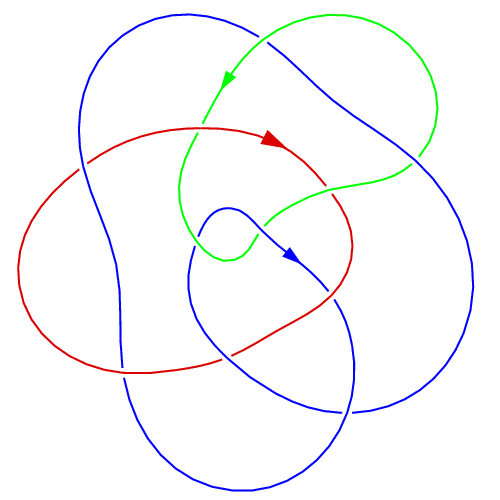
\includegraphics[width=\linewidth]{../data/link_mirror.png}
            \subcaption{lustro $mL$}
        \end{minipage}
        \begin{minipage}[b]{.32\linewidth}
            \centering
            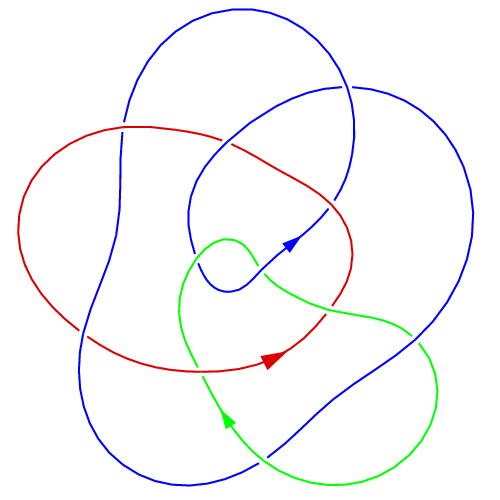
\includegraphics[width=\linewidth]{../data/link.png}
            \subcaption{przykładowy splot $L$}
        \end{minipage}
        \begin{minipage}[b]{.32\linewidth}
            \centering
            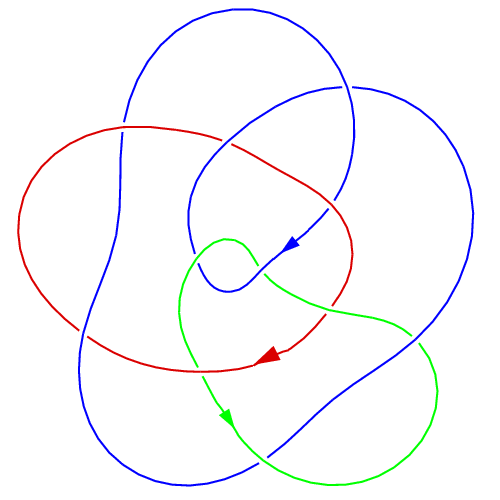
\includegraphics[width=\linewidth]{../data/link_reverse.png}
            \subcaption{rewers $rL$}
        \end{minipage}
    \end{figure}
\end{definition}

Na lewym obrazku odbiliśmy diagram względem poziomej prostej,
ale równie dobrze można po prostu zamienić każde nadskrzyżowanie na podskrzyżowanie.
Zauważmy, że wykonując powyższe operacje na węźle możemy otrzymać mniej niż czterech różne obiekty
($L$, $mL$, $rL$, $mrL$) -- na przykład trójlistnik jest własnym rewersem, ale nie lustrem.

\begin{definition}
    \index{węzeł!chiralny}
    \index{węzeł!odwracalny}
    \index{węzeł!zwierciadlany}
    Istnieje pięć typów symetrii węzłów:
    całkowicie chiralny albo skrętny (węzły $K$, $rK$, $mK$ są parami nierównoważne),
    odwracalny ($K \cong rK$),
    zwierciadlany ujemnie ($K \cong mrK$),
    zwierciadlany dodatnio ($K \cong mK$) oraz
    całkowicie zwierciadlany ($rK \cong K \cong mK$).
\end{definition}

Węzeł $9_{32}$ jest całkowicie skrętny.
Ósemka jest zwierciadlana, trójlistnik jest odwracalny, zaś $8_{17}$ to najprostszy przykład węzła nieodwracalnego.
Ten ostatni fakt jest jednak daleki od oczywistego -- sześćdziesiąt lat temu nie było pewne, czy węzły nieodwracalne w~ogóle istnieją.
W roku 1962 Ralph Fox wskazał kilku kandydatów do tego tytułu.
Hale Trotter odkrył rok później nieskończoną rodzinę nieodwracalnych precli (patrz \ref{trotter}).
Obecnie wiadomo, że prawie wszystkie węzły są nieodwracalne (\cite[s.~46]{murasugi96}).
Wszystkie węzły torusowe są skrętne.

Tait odnosił wrażenie, że zwierciadlane węzły mają parzysty indeks skrzyżowań,
ale Hoste (Thistlethwaite?) znalazł w~1998 kontrprzykład o~piętnastu skrzyżowaniach.
Jest on jedynym znanym nam dzisiaj.
Hipoteza Taita jest prawdziwa dla węzłów pierwszych, alternujących.

Poniższa tabela oparta jest (kolejno) o~ciągi
\href{https://oeis.org/A051766}{51766},
\href{https://oeis.org/A051769}{51769},
\href{https://oeis.org/A051768}{51768},
\href{https://oeis.org/A051767}{51767},
\href{https://oeis.org/A052400}{52400},
z bazy danych ``The On-Line Encyclopedia of Integer Sequences'' (OEIS).

\begin{table}[h]
    \centering
    \begin{tabular}{@{}*{20}l@{}} \toprule
        skrzyżowania & 3 & 4 & 5 & 6 & 7 & 8 & 9 & 10 & 11 & 12 & 13 & 14 \\ \midrule
        całkowicie skrętne & 0 & 0 & 0 & 0 & 0 & 0 & 2 & 27 & 187 & 1103 & 6919 & 37885 \\
        odwracalne & 1 & 0 & 2 & 2 & 7 & 16 & 47 & 125 & 365 & 1015 & 3069 & 8813 \\
        $-$ zwierciadlane & 0 & 0 & 0 & 0 & 0 & 1 & 0 & 6 & 0 & 40 & 0 & 227 \\
        $+$ zwierciadlane & 0 & 0 & 0 & 0 & 0 & 0 & 0 & 0 & 0 & 1 & 0 & 6 \\
        zwierciadlane & 0 & 1 & 0 & 1 & 0 & 4 & 0 & 7 & 0 & 17 & 0 & 41 \\
        \bottomrule
        \hline
    \end{tabular}
    \caption{Liczba węzłów o~poszczególnych typach symetrii}
    \label{tablica_wezlow}
\end{table}

Można wyróżnić jeszcze jeden rodzaj symetrii.

\begin{definition} \label{def_period}
    \index{węzeł!okresowy}
    Węzeł $K$ nazywamy $n$-okresowym, jeśli istnieje obrót $f \colon \R^3 \to \R^3$ o~kąt $2\pi/n$ wokół pewnej prostej $l$, rozłącznej z~węzłem, taki że $f(K) = K$.
\end{definition}

Trójlistnik jest 3-okresowy, węzeł $5_1$ 5-okresowy (widać to na standardowym diagramie) i~2-okresowy.
Tę drugą symetrię można dostrzec na diagramie realizującym indeks mostowy.

\begin{proposition}
    Zbiór wszystkich okresów jest niezmiennikiem węzłów.
\end{proposition}

Z~każdym węzłem okresowym związany jest inny, prostszy węzeł.
Niech $f$ będzie obrotem z definicji \ref{def_period}, zaś $p \colon \R^3 \to \R^3/f \simeq \R^3$ rzutem na przestrzeń ilorazową.
\index{węzeł!ilorazowy}
Wtedy $p(K)$ nazywamy \emph{węzłem ilorazowym}, zaś $K$ to jego $n$-krotne nakrycie.

Murasugi podał dwa warunki, które musi spełniać węzeł o~okresie $n = p^r$, gdzie $r$ jest liczbą pierwszą.
Do ich zrozumienia potrzebujemy prostej definicji.
Ustalmy półprostą, która nie jest styczna do węzła $K$, po czym zorientujmy ją oraz węzeł.
Indeksem zaczepienia $\lambda$ węzła $p(K)$ jest różnica między liczbą skrzyżowań dodatnich oraz ujemnych wzdłuż półprostej (bez znaku).

\begin{proposition}[warunek Murasugiego]
    \index{warunek Murasugiego}
    \label{murasugi_periodic}
    Niech $K$ będzie węzłem o~okresie $n = p^r$, gdzie $p$ jest liczbą pierwszą.
    Niech $J$ będzie jego węzłem ilorazowym, z~indeksem zaczepienia $\lambda$.
    Wtedy wielomian $\Delta_J$ jest dzielnikiem wielomianu $\Delta_K$ oraz istnieje pewna całkowita liczba $k$, taka że
    \[
        \Delta_K = \pm \Delta_J^n \left(1 + t + t^2 + \ldots + t^{\lambda - 1}\right)^{n-1} \mod p.
    \]
\end{proposition}

Dowód to, jak zwykle, mozolne operacje na macierzach.

% Koniec podsekcji Lustro i~rewers

\subsection{Suma niespójna i~suma spójna} % (fold)
\label{sub:knot_sum}
Suma spójna węzłów to szczególny przypadek sklejenia dwóch rozmaitości wzdłuż brzegu.

\begin{definition}[suma niespójna]
    \index{suma!niespójna}
    Niech $L_1$ oraz $L_2$ będą splotami, które leżą po różnych stronach ustalonej płaszczyzny w przestrzeni $\R^3$.
    Teoriomnogościową sumę $L_1 \sqcup L_2$ nazywamy sumą niespójną splotów.
\end{definition}

\begin{definition}[suma spójna]
    \index{suma!spójna}
    Niech $K_1, K_2$ będą zorientowanymi węzłami.
    Natnijmy każdy z nich w dwóch punktach tego samego krótkiego łuku, a następnie zszyjmy dwoma łukami, które nie przecinają już istniejących, jak na obrazku.
    Otrzymany węzeł nazywamy sumą spójną węzłów $K_1$ oraz $K_2$.
    \[
        \begin{tikzpicture}[baseline=-0.65ex,scale=0.1]
        \begin{knot}[clip width=5, flip crossing/.list={5}, ignore endpoint intersections=false,]
            \strand[thick] (-3.5, -3.5) [in=down, out=up] to (3.5, 3.5);
            \strand[thick] (3.5, 3.5) [in=right, out=up] to (-4.5, 10);
            \strand[thick] (-4.5, 10) [in=up, out=left] to (-10, 3.5);
            \strand[thick] (-10, 3.5) to (-10, -3.5);
            \strand[thick] (-10, -3.5) [in=left, out=down] to (-4.5, -10);
            \strand[thick] (-4.5, -10) [in=down, out=right] to (3.5, -3.5);
            \strand[thick] (3.5, -3.5) [in=down, out=up] to (-3.5, 3.5);
            \strand[thick] (-3.5, 3.5) [in=left, out=up] to (4.5, 10);
            \strand[thick] (4.5, 10) [in=up, out=right] to (10, 3.5);
            \strand[thick, -Latex] (10, 3.5) to (10, -3.5);
            \strand[thick] (10, -3.5) [in=right, out=down] to (4.5, -10);
            \strand[thick] (4.5, -10) [in=down, out=left] to (-3.5, -3.5);
            \node at (0, -15) {$K_1$};
        \end{knot}
        \end{tikzpicture}
        \shrap
        \begin{tikzpicture}[baseline=-0.65ex,scale=0.1]
        \begin{knot}[clip width=5, flip crossing/.list={6}, ignore endpoint intersections=false,]
            \strand[thick] (-3.5, -3.5) [in=down, out=up] to (3.5, 3.5);
            %\strand[thick] (3.5, 3.5) [in=right, out=up] to (-4.5, 10);
            %\strand[thick] (-4.5, 10) [in=up, out=left] to (-10, 3.5);
            \strand[thick] (-10, -3.5) [in=left, out=up] to (0, 6.5);
            \strand[thick, Latex-] (-10, -3.5) [in=left, out=down] to (-4.5, -10);
            \strand[thick] (-4.5, -10) [in=down, out=right] to (3.5, -3.5);
            \strand[thick] (3.5, -3.5) [in=down, out=up] to (-3.5, 3.5);
            %\strand[thick] (-3.5, 3.5) [in=left, out=up] to (4.5, 10);
            %\strand[thick] (4.5, 10) [in=up, out=right] to (10, 3.5);
            \strand[thick] (10, -3.5) [in=right, out=up] to (0, 6.5);
            \strand[thick] (10, -3.5) [in=right, out=down] to (4.5, -10);
            \strand[thick] (4.5, -10) [in=down, out=left] to (-3.5, -3.5);
            %
            \strand[thick] (-3.5, 3.5) [in=left, out=up] to (0, 10);
            \strand[thick] (3.5, 3.5) [in=right, out=up] to (0, 10);
            \node at (0, -15) {$K_2$};
        \end{knot}
        \end{tikzpicture}
        =
        \begin{tikzpicture}[baseline=-0.65ex,scale=0.1]
        \begin{knot}[clip width=5, flip crossing/.list={5, 22, 23}, ignore endpoint intersections=false,]
            \strand[thick] (-18.5, -3.5) [in=down, out=up] to (-11.5, 3.5);
            \strand[thick] (-11.5, 3.5) [in=right, out=up] to (-19.5, 10);
            \strand[thick] (-19.5, 10) [in=up, out=left] to (-25, 3.5);
            \strand[thick] (-25, 3.5) to (-25, -3.5);
            \strand[thick] (-25, -3.5) [in=left, out=down] to (-19.5, -10);
            \strand[thick] (-19.5, -10) [in=down, out=right] to (-11.5, -3.5);
            \strand[thick] (-11.5, -3.5) [in=down, out=up] to (-18.5, 3.5);
            \strand[thick] (-18.5, 3.5) [in=left, out=up] to (-10.5, 10);
            \strand[thick] (-10.5, 10) [in=left, out=right] to (-5, 2);
            \strand[thick, -Latex] (-5, 2) to (-5+6, 2);
            \strand[thick] (5, 2) to (-5+6, 2);
            \strand[thick] (3, -2) to [in=left, out=right] (10.5, -10);
            \strand[thick, -Latex] (3, -2) to (0, -2);
            \strand[thick] (-5, -2) to (0, -2);
            \strand[thick] (-5, -2) [in=right, out=left] to (-10.5, -10);
            \strand[thick] (-10.5, -10) [in=down, out=left] to (-18.5, -3.5);
            %%%
            \strand[thick] (11.5, -3.5) [in=down, out=up] to (18.5, 3.5);
            \strand[thick] (-10 +15, 2) [in=left, out=right] to (15, 6.5);
            \strand[thick] (10.5, -10) [in=down, out=right] to (18.5, -3.5);
            \strand[thick] (18.5, -3.5) [in=down, out=up] to (11.5, 3.5);
            \strand[thick] (25, -3.5) [in=right, out=up] to (15, 6.5);
            \strand[thick] (25, -3.5) [in=right, out=down] to (19.5, -10);
            \strand[thick] (19.5, -10) [in=down, out=left] to (11.5, -3.5);
            \strand[thick] (11.5, 3.5) [in=left, out=up] to (15, 10);
            \strand[thick] (18.5, 3.5) [in=right, out=up] to (15, 10);
            %%%
            \node at (0, -15) {$K_1 \shrap K_2$};
        \end{knot}
        \end{tikzpicture}
        \]
\end{definition}

Uogólnieniem sumy spójnej oraz (nieopisanej w~naszej pracy) operacji \emph{plumbing} jest suma Murasugiego, dobrze wyjaśniona w~czwartym rozdziale książki \cite{kawauchi96}.
W topologii rozważa się podobną operację dla dwóch $n$-wymiarowych rozmaitości: z~każdej z nich usuwa się kulę, po czym skleja wzdłuż brzegu kuli.
Kiedy zajmujemy się węzłami, nie interesuje nas jednak struktura rozmaitości (gdyż każdy węzeł jest równoważny z okręgiem), ale zanurzenie w~otaczającą przestrzeń.

Ważna jest orientacja składników:
suma dwóch trójlistników może być,
w zależności od ich orientacji,
węzłem babskim\footnote{Nazewnictwo pochodzi od żeglarzy, nie matematyków. Z angielskiego \emph{granny knot}, \emph{square knot}.} lub prostym.
Fox pokazał w~1952 roku,
że dopełnienia tych dwóch węzłów nie są homeomorficzne.
Suma przeciwnie skręconych trójlistników jest plastrowa
(definicja \ref{def:slice_knot}),
natomiast tak samo skręconych -- nie.

\begin{proposition}
    Suma spójna jest dobrze określonym działaniem.
\end{proposition}

Suma spójna nie jest dobrze określona dla splotów:
nie istnieje kanoniczny wybór, które ogniwa łączyć ze sobą.

\begin{proof}
    Niech dane będą węzły $K_1$ oraz $K_2$
    oraz dwa różne łuki $\gamma_1$, $\gamma_2$,
    których można użyć do konstrukcji sumy spójnej.
    Skurczmy $K_1$, przeciągnijmy najpierw przez łuk $\gamma_1$, a~następnie wzdłuż węzła $K_2$.
    Teraz wystarczy odwrócić ten proces z~$\gamma_2$ w~miejscu $\gamma_1$.
\end{proof}

\begin{proposition}
    Suma spójna jest działaniem łącznym oraz przemiennym.
    Niewęzeł stanowi jej element neutralny.
\end{proposition}

Prosty dowód tego faktu pozostawiamy Czytelnikowi.
W języku algebry mówimy, że węzły z~sumą spójną tworzą półgrupę (tak jak liczby naturalne z działaniem dodawania).
Dużo później pokażemy, że działaniu $\shrap$ brakuje elementów przeciwnych, więc ta struktura algebraiczna nie jest grupą.

\begin{proposition}
    Jeśli $K \shrap L = \Unknot$, to $K = L = \Unknot$.
\end{proposition}

\begin{proof}[Niedowód]
    Technika ta zwana jest szwindlem Mazura.
    Załóżmy, że $K \shrap L = \Unknot$ i~dopuśćmy wyjątkowo węzły dzikie.
    Skonstruujmy sumę $K \shrap L \shrap K \shrap \ldots$,
    przy czym kolejne składniki powinny zmniejszać się,
    aby ich suma nadal była węzłem.
    Wtedy
    \begin{align*}
        K & \simeq K \shrap [(L \shrap K) \shrap (L \shrap K) \ldots] \\
         & \simeq (K \shrap L) \shrap (K \shrap L) \shrap \ldots
         \simeq \Unknot \shrap \Unknot \shrap \ldots
         \simeq \Unknot.
    \end{align*}
    Analogicznie pokazujemy, że $L \simeq \Unknot$.
\end{proof}

Prawdziwy dowód oparty jest na topologii algebraicznej, stanowi bezpośredni wniosek z~faktów \ref{genus_one} oraz \ref{genus_sum}.

Półgrupę węzłów z~operacją sumy spójnej można ulepszyć do grupy na dwa sposoby:
albo poprzez zmianę działania, w~jakie jest wyposażona,
albo osłabiając definicję węzłów równoważnych.
Drugi pomysł jest dużo lepszy niż pierwszy.
Na początku lat pięćdziesiątych J. Milnor wprowadził do matematyki pojęcie zgodności
(z angielskiego \emph{concordance}), które zastąpiło zwykłą równoważność.
Element neutralny nowej grupy to węzły plastrowe, ich opis leży w~sekcji \ref{sec:slice}.
Zagadnienia te zakorzenione są w~czterowymiarowej topologii.

% Koniec podsekcji Suma niespójna i~suma spójna

% Koniec sekcji Operacje na węzłach
